\documentclass[letterpaper,11pt]{article}
\usepackage[utf8]{inputenc}
\usepackage{a4wide}
\usepackage{amsfonts}
\usepackage[utf8]{inputenc}
\usepackage[english]{babel}
\usepackage{amsthm}
\usepackage{scalerel}
\usepackage{hyperref}
\usepackage{amsmath}
\usepackage{enumitem}


\newtheorem{definition}{Definition}
\newtheorem{theorem}{Theorem}
\newtheorem{lemma}{Lemma}


\newcommand{\sk}{\ensuremath{\mathsf{sk}}} %secret key
\newcommand{\pk}{\ensuremath{\mathsf{pk}}} %public key
\newcommand{\verify}{\ensuremath{\mathsf{Verify}}}
\newcommand{\prove}{\ensuremath{\mathsf{Prove}}}
\newcommand{\divi}{\ensuremath{\mathsf{Divide}}}
\newcommand{\recons}{\ensuremath{\mathsf{Reconstruct}}}
\newcommand{\pv}{\ensuremath{\mathcal{P}V}}
\newcommand{\V}{\ensuremath{\mathcal{V}}}
\newcommand{\bb}{\ensuremath{\mathbb{B}}} %blob
\newcommand{\bh}{\ensuremath{B_{head}}} %block header
\newcommand{\mprf}{\ensuremath{\pi^{mt}}} %merkle proof
\newcommand{\vcheck}{\ensuremath{\#V\mathsf{check}}} %number of validity check
\newcommand{\runav}{\ensuremath{r_{a}}}
\newcommand{\rinv}{\ensuremath{r_{f}}}
\newcommand{\pr}{\ensuremath{\mathsf{Pr}}} %probability




\title{Availability and Validity}


\begin{document}
\date{}
\maketitle

\section{Definitions}

\paragraph{Notations} $\V= \{V_1,V_2,...,V_n\}$ is the validator set consisting of validators $V_i$. $\pv$ is a set of parachain validators and $\pv \subset \V$. For the sake of distinction, we denote parachain validators by $PV_i \equiv V_i$.

\begin{definition}[Blob]
A blob is a tuple $(B, \pi, M)$ where $B$ is the parachain block, $\pi$ is the validity proof of $B$ and $M$ is the outgoing messages from that parachain.
\end{definition}


\begin{definition}[Block Header]\label{def:header}
Block header is a summary of the block $B$ which links to $B\in PC$ and includes all the signatures by parachain validators who claims its validity. There exists a function $\recons$ which takes the block header $B_{head}$ and block data $B_{data}$ as an input and outputs $B$ which $B_{head}$ is linked to. 
\end{definition}



\begin{definition}[Erasure Code]\label{def:erasure}
Erasure code consists of two algorithms: $\divi_k$ and $\recons$ Given data $D$, the algorithm $\divi$ outputs $n$ pieces $d_1,d_2,...,d_n$ and given $k$ out of $n$ pieces, $\recons$ outputs $D$.  

\end{definition}

In other words, erasure code divides  data into $n$ pieces and at least $k$ out of $n$ pieces are enough the construct the data.

In the availability and validity protocol in Section \ref{sec:protocol}, parachain validators divide a blob into $n$ pieces. These $n$ pieces corresponds the $B_{data}$ in Definition \ref{def:header} and so the $\recons$ algorithm in Definition \ref{def:header}  corresponds the $\recons$ algorithm of the erasure code in Definition \ref{def:erasure}.








\subsection{Security Model}


%Think it again
%\begin{definition}[Risk Value]
%Given a total stake $S$ and slashing value $x$, the risk value is defined as $p\frac{x}{S}$ where $p$ is the probability of getting caught.
%\end{definition}

The active parties in availability and validity scheme are validators, parachain validators, fishermen and collators. 




\begin{itemize}

\item Parachain validators are responsible to validate a blob. They can be malicious.
\item Collators are the full nodes of parachain and provide a PoV blob to the responsible parachain validators. They can be malicious and collude with parachain validators.
\item Validators are responsible of maintaining relay chain and finalizing the blocks in the relay chain. A validator can be also a parachain validator. 
\item Fishermen inspects any malicious activity. If any exists they announce and prove it.  



\end{itemize}

In our security model, we assume that all parties except fishermen can be malicious. Given $|V| = n = 3f + 1$, at most number of $f$ validators can be malicious.


\begin{definition}[Proof of Validity (PoV)]\label{def:pob}
PoV consists of two algorithms $\prove$ and $\verify$:
\begin{itemize}
    \item $\prove$  takes the block $B$, the parachain $PC$ and the outgoing messages from $PC$ as an input and outputs the proof $\pi$.
    \item $\verify$  takes the blob $(B,\pi,M)$ as an input and outputs 1 (valid) or 0 (invalid).
\end{itemize}
\end{definition}
\paragraph{Correctness of PoV:} PoV is correct if for all $B \in PC$ and $M$, $\verify(B,\pi,M)\rightarrow 1$ where $\prove(B, PC,M)\rightarrow \pi$.

\paragraph{Security of PoV:} PoV is secure if an adversary generates a blob $(B,\pi,M)$ for a parachain $PC$ where  $\verify(B,\pi,M) \rightarrow 1$ and $B \notin PC$ with a negligible probability.


We note that $B\in PC$ (resp. $B \notin PC$) means that the block $B$ is a valid (resp. invalid) block for a parachain $PC$.


\begin{definition}[Unavailable Block]\label{def:unavail}
A block is unavailable if less than $k$ erasure code of its blob obtained by honest validators.
\end{definition}


\begin{definition}[Security of Availability]
Assume that  at most number of $f$ validators are corrupted. If the probability of having a finalized block in the relay chain which includes an unavailable block is negligible, then the availability protocol is secure against malicious validators.
\end{definition}

%More formal definition
\begin{definition}[Security of Validity]
Assume that  at most number of $f$ validators are corrupted. If the probability of having a finalized block in the relay chain which includes the header of an invalid block is less than a risk value, then the validity protocol is secure against malicious validators.
\end{definition}







\section{Availability and Validity Protocol}
\label{sec:protocol}

The protocol consists of two phases ``Parachain phase'' and ``Relay Chain Phase''. The parachain phase is executed between collators and parachain validators. In the end of this phase, the parachain validators validate the block and provide its erasure code pieces to the validators. Then, the relay chain phase begins. If the parachain phase is executed correctly, then the relay chain phase includes extra validation of a parachain block, adding the block header to the relay chain and finalizing that relay chain block. Otherwise, unavailability protocol is run between validators. The details are as follows: 

\paragraph{Parachain Phase:} This phase is between parachain validators and collators of the corresponding parachain.

\begin{itemize}
    \item For each parachain block $B$, a collator runs the $\prove(B,PC,M)$ and obtains the proof $\pi$ for the validity of  block $B$. Then, he sends the blob $\bb = (B,\pi,M)$ to the corresponding parachain validators to show that the block is valid and can be added to the relay chain. 
    
    \item Each parachain validator $PV_i$ checks the validity of the block by running the $\verify$ algorithm for the blob $\bb$. If it outputs 0, they ignore the block and store the block as invalid. Otherwise, $PV_i$ runs the $\divi(\bb)$ to obtain the erasure code pieces $\mathcal{D} = \{d_1,d_2,...,d_n\}$ of $\bb$.
    
    \item $PV_i$ constructs a Merkle tree  with  leaves $d_1,d_2,...,d_n$. Let us denote the root of the Merkle tree by $r$. At the end, $PV_i$ signs for each validator $V_j$ the message $(d_j, r, \mprf_i, B_{info})$ and gives each signature $\sigma_i^j$ to the distributor parachain validator. Here, $\mprf_i$ is the proof that shows that $d_i$ is one of the leaves of the Merkle tree with the root $r$ and $B_{info}$ is identifying information of $B$. We note that the distributor can be selected randomly or in order. Each parachain validator also gives the erasure code piece to at least one (trusted) collator in order to backup the piece.
\end{itemize}


 


\paragraph{Relay Chain Phase:} This phase is to make sure that a valid and available block's header is in the relay chain. 

\begin{itemize}
    \item After receiving the signatures from parachain validators in the parachain phase, the distributor sends  for each validator $V_j$ all signatures  $\{\sigma_j^k\}_{PV_k \in \pv'} $ where $\pv' \subseteq \pv$ representing the set of parachain validators who sent a signature for $V_j$. 

    \item If $V_j$ receives at least $\kappa$ signatures for $B$, it adds it to the block list which keeps the data to be included to the relay chain. Later on, if this validator is the designated validator in BABE to produce the block, it creates block headers $\bh$ (Definition \ref{def:header}) for the blocks in the block list. $\bh$ including $\{\sigma_j^k\}_{PV_k \in \pv'} $.  These signatures are necessary to show which parachain validators approve for $B$. Then, he produces the relay chain block which includes the header. See \href{http://research.web3.foundation/en/latest/polkadot/BABE/Babe/}{BABE} for details.

    \item At the same time, each validator $V_j$ examines  each block in the relay chain if it includes unavailable block headers. If $V_j$ sees a block header $\bh$ in a block of the best relay chain whose erasure code piece $d_j$ is not received by $V_j$ (unavailable code piece), then he asks for it first from parachain validators. If a parachain validator sends valid $d_j, r, \mprf_j $, then the protocol ends. Otherwise, it asks for it from collators of the corresponding parachain. If $V_j$ receives a valid $d_j, r, \mprf_j $, the protocol ends. If $V_j$ does not receive any response in $\Delta T$ time after seeing $\bh$, he runs the unavailability protocol in Section \ref{sec:unavail}.

\end{itemize}

\subsection{Unavailability Protocol}
\label{sec:unavail}
If a validator could not obtain the missing piece in $\Delta T$ time (availability grace period) after seeing a block header $B_{head}$ in a block of the relay chain, then he announces the unavailability of this piece. As soon as receiving an unavailability announcement, the assigned validator sends the erasure code piece with the proof, if he has it. The details of how the assigned validator is selected and how he obtains the erasure codes are given in Section \ref{sec:validitycheck}. If any validator sees at least $f+1$ unavailability announcements from different validators, then he does not vote to finalize the block which includes a block header whose pieces are missing  because it is a sign that the parachain validators have not properly completed availability protocol. If $2/3$ of the validators announce unavailability of a piece, the parachain validators who signed for that block are slashed. 

%TODO slashing process



\subsection{Validity Check}
\label{sec:validitycheck}
With the unavailability protocol, we can detect the block headers whose pieces are missing. Beyond this, we also need to detect whether invalid block headers are in the relay chain blocks. For example, if all parachain validators are malicious, they can sign for an invalid block. We can catch this only by reconstructing the blob with the available pieces. In the validity check protocol, we describe how extra validators (different from parachain validator) are assigned to check the validity of blocks and how malicious activities are detected.


We first give some parameters before giving the details of the protocol.
The first parameter $\vcheck$ defines the total number of validator checks needed for a block header.

$$\vcheck = |\pv| + \mu +\lceil \runav + \rinv \rceil$$

Here, $\mu$ specifies the minimum number of checks, $\runav$ is the unavailability report factor from collators and $\rinv$ is the invalidity report factor from fishermen who claim invalidity for the relevant block. 


%Here, $\mu$ specifies the minimum number of checks, $\runav$ is the unavailability report factor which is the constant $c_a$ multiplied with the rate of the unavailability report in the last 1000 blocks.
%$\rinv$ is the invalidity report factor which is the constant $c_f$ multiplied with the relative stake of fishermen who claim invalidity for the relevant block. 




There are a three-factor validity check during the availability protocol:


\begin{enumerate}

      
    \item \textbf{Fisherman Check:} All fishermen collect blobs from collators in order to check the validity all the time. Whenever they discover an invalid block, they announce it to the validators by signing their claim. These claims are added to the block list by the validators. So, these claims are going to be in the relay chain. They do not provide any proof. If their claims are wrong then they are slashed. Otherwise, they are rewarded. The correctness of the fishermen claims are determined with the validity check protocol.
    
    \item \textbf{Parachain Validator Check:} All parachain validators check the validity of the block as described in the parachain phase of the availability protocol. If one parachain validator $PV_i$ sees that an invalid block header is in a block of the best relay chain, then he announces the invalidity. If a parachain validator has never seen the blob of the block header in the relay chain or he does not sign for that block, he runs the extra validity check protocol given below.
    
    \item \textbf{Non-Parachain Validator Check:} The extra validity checks are done by the non-parachain validators. Now, we explain how these validators are selected.
    
    \paragraph{Selection:} The selection process is private and no one knows the selected ones until they make it public. Assume that there exists $m$ parachains in Polkadot. Each validator $V_j$ checks first the following if required extra check is more than $n/m$ (i.e., $\mu + \lceil r_a + r_f \rceil \geq n/m$): 
    
    \begin{equation}\label{cond:mod}
        ID_{PC} = \mathtt{VRF}_{\sk^v_{j}}(r_{t}) \mod m    
    \end{equation}
     Here, $ID_{PC} \in \mathbb{N}$ is the identifier of a parachain $PC$ and $r_{t}$ is the VRF randomness of the block producer of slot $t$ in the relay chain (See \href{http://research.web3.foundation/en/latest/polkadot/BABE/Babe/}{BABE} for the details of $r_t$). For the current time $T$ where $T > \Delta T$, if  less than $\vcheck$ amount of checks are completed with condition (\ref{cond:mod}) or $\mu + \lceil r_a + r_f \rceil < n/m$ , each validator $V_j$ checks the following condition:
     \begin{equation}\label{cond:time}
        H(ID_{PC} || \mathtt{VRF}_{\sk^v_j}(r_t)) < \frac{\mu + \lceil r_a + r_f \rceil - \theta}{|\V|-|\pv|}+\tau  
    \end{equation}
    
      where $\tau = T- \Delta T$ and $H$ is a hash function that maps a value between 0 and 1. Here, if $\mu + \lceil r_a + r_f \rceil \geq n/m$, $\theta$ is the number of validators in condition (\ref{cond:mod}) for $ID_{PC}$. Otherwise, $\theta = 0$.
    
    However, if a block producer produces multiple blocks with the same VRF randomness $r_t$ (equivocation), then a validator $V_j$ is selected for the extra check if one of the  below two conditions together with (\ref{cond:mod}) and (\ref{cond:time}) are satisfied:
    
    
    \begin{equation}\label{cond:modequiv}
         ID_{PC} = \mathtt{VRF}_{\sk^v_{j}}(r_{t}||H_B) \mod m
    \end{equation}
    
    \begin{equation}\label{cond:equiv}
         H(ID_{PC} || \mathtt{VRF}_{\sk^v_j}(H_{B})) < \frac{\vcheck - |\pv|}{|\V|-|\pv|}   
    \end{equation}
    
     where $H_B$ is the hash of the relay chain block whose VRF randomness is $r_t$. Remark that we have greater number of checks for equivocation because it is a sign of malicious activity. Malicious validators can see who is in condition (\ref{cond:mod}) or (\ref{cond:time}) and if there is  no honest validator with the conditions (\ref{cond:mod}) or (\ref{cond:time}), they can equivocate which includes an invalid block. Therefore, we need different conditions than the condition (\ref{cond:mod}) and the condition (\ref{cond:time}).
    
    When $V_j$ satisfies the condition (\ref{cond:mod}), (\ref{cond:time}), (\ref{cond:modequiv}) or (\ref{cond:equiv}), $V_j$ has a right to check the validity. For this, it follows the extra validity check protocol.
    
    We note that if number of $\vcheck$ validators satisfy the condition (\ref{cond:mod}) or (\ref{cond:time} ) for a parachain with the identifier $ID_{PC}$ and no equivocation exist, then satisfying condition (\ref{cond:modequiv}) or (\ref{cond:equiv}) does not get rewarded.
    
\end{enumerate}


\paragraph{Extra Validity Check:}
An assigned validator $V_j$  asks for the blob for the extra validity check or the erasure code pieces in the following order until receiving all information to check the validity of the block header:
\begin{enumerate}
    \item Parachain validators who signed for it: asked for the blob
    \item Other parachain validators who did not sign for it: asked for the blob
    \item Validators: asked for the erasure code piece with the proof. Assuming that $V_j$ has a set $\mathcal{D}'$ of a correct erasure codes where $|\mathcal{D}'|<k$. He asks for at least number of $k-|\mathcal{D}'|$ pieces in $\mathcal{D}\setminus \mathcal{D}'$ from the validators.
    
    \item Collators: asked for the erasure codes or the blob. We note that $V_j$ can ask for the blob or the erasure code, if he is connected to the collators network.
    
\end{enumerate}

In the end,  if $V_j$'s attempt in option 1 and 2 above is unsuccessful and  obtains all missing pieces instead of blob $\bb$, he adds them to the set $\mathcal{D}'$ and reconstructs  $\bb = (B,\pi,M)$ with the algorithm $\recons(\mathcal{D}')$. 

In any case, either obtaining $\bb$ from $PV$s or the reconstruction algorithm, $V_j$ checks the validity of the block by  running  $\verify(\bb)\rightarrow b$.
\begin{itemize}
    \item if $b = 0$ (the blob is invalid), $V_j$ signs that the block is invalid. Whenever a validator receives a valid signature from another validator saying that the block is invalid, this validator obtains the blob  the same way that extra validators obtain and follow the same process.
    \item if $b = 1$ (the blob is valid), $V_j$ signs that the block is valid. $V_j$ also  runs the $\divi((B,\pi,M))$ to obtain the erasure codes $\mathcal{D} = \{d_1,d_2,...,d_n\}$ and constructs a Merkle tree  whose leaves are $d_1,d_2,...,d_n$. In the end, he gives away the missing piece of the validator with the Merkle tree proof whenever a validator announces unavailability. 
\end{itemize}


In the end of the validity protocol, if at least $f+1$ signatures are given by the validators saying that the block is invalid, then it is considered as invalid.
\subsection{Slashing and Rewarding}

\underline{\textbf{Fisherman}} 

\emph{Slashing:} If at least $\vcheck$ validators sign saying that the block is valid, then fishermen with the claim saying the block is invalid are slashed. All the claims from these fishermen are ignored in future.

\emph{Rewarding:} If $f+1$ validators sign to say the block is invalid, the  fishermen with the claim saying that the block is invalid are rewarded.

%TODO MORE DETAILS

\noindent\underline{\textbf{Validators}}

\emph{Slashing:} If at least $f+1$ validators sign for the invalidity of a block and less than $f+1$ validators sign for the validity of the block, then we slash all validators who signed for the validity.

If at least $f+1$ validators sign for the validity of a block and less than $f+1$ validator sign for invalidity, we slash the ones who signs for the invalidity.

We note that $f+1$ validity signatures and $f+1$ invalidity signatures are not possible given that at most $f$ validators are malicious and proof of block algorithms  are correct (See Definition \ref{def:pob}).

\emph{Rewarding:} All parachain validators and extra validators who signed for the final decision (either valid or invalid) of a block receive a reward. 

Eligibility of the reward can be easily checked for the parachain validators and extra validators who satisfies the conditions when $\tau = 0$. Latter, we just need to verify the VRF proof.
However, it is not easy to verify the condition for $\tau > 0$, because this value is subjective. Therefore, we may not need to be very precise for this $\tau$ value, if the signature of the validator is correct.

%\section{Security of Availability and Validity}


\begin{theorem}[Availability]
Assuming the Merkle tree constructed from collision resistant hash functions and a block in GRANDPA can be finalized with at least $2f+1$ votes, then the availability protocol is secure.
\end{theorem}

\begin{proof}
Assume that an unavailable block is finalized. It means that this finalized block includes a block header of which at most $f$ honest validators has the correct erasure code piece (See Definition \ref{def:unavail}). If this block is finalized, it means that
\begin{itemize}
    \item either not all honest validator who does not have the erasure code piece announce the unavailability. If they would announce it, since their number is at least $2f+1 - f =f+1$ (i.e., honest parties - honest parties who do not have the erasure code), the other honest parties do not finalize it and malicious parties do not have enough number to finalize it. Therefore, we can assume that there is at least one honest party who do not announce the unavailability of its erasure code in this case, because he thinks that he has one but actually it is not correct. If there exists a one honest party who has incorrect erasure code, but having the proof that it is correct (provided by parachain validators), then it means that the collision resistance assumption of Merkle tree is broken. 
    
    \item or  $f+1$ parties announces unavailability it means that GRANDPA finalize the block with at most $2f$  parties. So, this implies that the security of GRANDPA is broken by finalizing a block with less than $2f+1$ votes.
\end{itemize}

Since the GRANDPA is secure and the Merkle tree is collision resistant, the unavailability protocol is secure.
\end{proof}

\begin{theorem}[Validity]
\label{thm:valid}
Assuming that the availability protocol is secure, the signature scheme is EF-CMA secure, the hash function $H$ in Conditions (\ref{cond:time}) and  (\ref{cond:equiv}) is a random oracle, the PoV protocol is secure and correct (Definition \ref{def:pob}), the VRF is secure and a block in GRANDPA can be finalized with at least $2f+1$ votes then the invalid block is finalized in the relay chain with probability less than risk probability.
\end{theorem}

\begin{proof}(Sketch)
TODO: Security reduction, Rewrite the security arguments


If there is one honest $PV$ and there is not any $f+1$ unavailability report, then at least $2f$ of the honest parties has the piece. It means that $PV$ can collect all the pieces from the honest parties in order to reconstruct the blob and check its validity. Therefore, if there is at least one honest party in $PV$, it can detect the invalidity and announces it. In the end, we will have more than $f$ invalidity signatures since the other parties also check invalidity after seeing the signature saying that the block is invalid.

Therefore, we analyze the case where all parachain validators are malicious. 
If there is at least one honest validators who is assigned for extra validity check then the same case happens as having at least one honest parachain validators. Therefore, we need to find out the probability of having all parachain and extra-check validators are malicious given that all parachain validators are malicious. 

There are three cases that the extra check validators are selected: Either with only condition (\ref{cond:mod}) or with condition (\ref{cond:mod}) and (\ref{cond:time}) or with condition (\ref{cond:equiv}). Let's analyze the success of malicious validators in these three cases. Below, $\mu' = \mu+\lceil \runav + \rinv \rceil $ which is the required number of non-parachain validator validity check and $f' < n/3 - n/m$ is the number of non-parachain malicious validators and  $|PV| = n/m = nc$ where $c 1/n$. 

$$\pr[\text{Cond. (\ref{cond:mod})}] =\pr[\text{Cond. (\ref{cond:modequiv})}] = p_{vrf} = \frac{1}{m}$$
$$\pr[\text{Cond. (\ref{cond:time}) at time } \tau] = p_\tau =  \frac{\mu'}{n - nc} + \tau $$
$$\pr[\text{Cond. (\ref{cond:equiv}) }] = \frac{\mu'}{n - nc} $$


%Remark that  with condition (\ref{cond:mod}), we can guarantee that there will be $n/m$ extra validator check. Therefore, if $n/m$ malicious validators do not satisfy the condition (\ref{cond:mod}), then their invalid block is always caught because it means there is at least one honest validator satisfying the condition (\ref{cond:mod}). Therefore, the attacks below are executed when $n/m$ malicious validators satisfy the condition (\ref{cond:mod}). 
\begin{enumerate}


    \item The malicious validators generate an invalid block when they see that at least $\mu'$ malicious validators satisfy the condition (\ref{cond:mod}). This can happen with probability
    
    \begin{equation}\label{eq:attack1cond}
        \sum_{i = \mu'}^{f'}\binom{f'}{i}\frac{1}{m^{i}}(1-\frac{1}{m})^{f'-i}    
    \end{equation}
     which is not negligible. When this happens, their attack succeeds if no honest validator satisfies the condition (\ref{cond:mod}). Then, the attack probability is the following:
	
	\begin{align}\label{eq:nocond1}
	\pr[\mathsf{attack1}] &= \pr[\text{no honest satisfies (\ref{cond:mod})}] \\ \nonumber
									 & \leq   (1-\frac{1}{m})^{2n/3} \\ \nonumber
									 & \leq  e^{-2n/3m} 
	\end{align}
	
	
% 	\item If $\mu' \leq n/m$, the malicious validators generates an invalid block and their attack succeeds since 
	
% 	\begin{align}\label{eq:nocond1}
% 	\pr[\mathsf{attack1}] &=  \binom{f'}{n/m}\frac{1}{m^{n/m}} 
% 	\end{align}

	
    \item The malicious validators generate an invalid block. In this case their attack succeeds if no honest validator satisfies the condition (\ref{cond:mod}) and the condition \ref{cond:time} until a time where at least $\mu'$ malicious validators satisfy the condition \ref{cond:time}. 
    For simplicity, we divide time in discrete values $[\tau_0 = 0, \tau_1 =u, \tau_2 = 2u, ..., \tau_k = ku]$. $\tau_k$ can be computed by malicious validators before the validation process begins. In any case, the only way not to be caught is not to have any honest extra-check validator until $ku$. The probability of this attack is the following:
    
    
    
    \begin{align}\label{eq:attack2}
        \pr[\mathsf{attack2}] &= \pr[\mathsf{attack1}]\prod_{i = 0}^k(1-p_{\tau_i})^{2f+1} \nonumber \\
        &\leq  e^{-2n/3m} \prod_{i = 0}^k (1 - \frac{\mu'+\tau_in(1-c)}{n(1-c)})^{\frac{2n}{3}} \nonumber\\
        &=  e^{-2n/3m} \exp(\sum_{i = 0}^k -\frac{2}{3}\frac{\mu' + \tau_in(1-c)}{1-c}) \nonumber\\
        & = \exp(-2/3(\frac{n}{m}+\frac{(k+1)\mu'}{1-m/n}+ nu\frac{k(k+1)}{2})
    \end{align}
    
    
    % \begin{align}
    %     \pr[\mathsf{attack 2}] \leq \pr[\mathsf{attack }1]\nonumber
				% 						  & = \frac{e^{-2c/3}}{m^{\mu'}} \prod_{i}^k(1-(\frac{\mu'}{n - nc} + \tau_i ))^{2n/3} \leq (1-p_{\tau_0})^{2f+1}\\ &\leq (1-\frac{1+c'_f}{n(1-c)}) ^{\frac{2}{3}n} \nonumber \\
    %     & \leq e^{-2/3\frac{1+c_f}{1-c}} \nonumber
    % \end{align}
    
    
    \item In this attack, the adversary equivocates the block. Here, we can assume that the adversary knows who satisfies the condition (\ref{cond:mod}) since if the malicious validator is the block producer, he first produces the block and sees who validates this block. If no honest validator checks it with condition (\ref{cond:mod}), he equivocates it.  We know that probability of no honest party satisfies the condition (\ref{cond:mod}) is given in  inequality (\ref{eq:nocond1}). When this happens, the attack succeeds if no honest party satisfies the condition (\ref{cond:modequiv}) and (\ref{cond:equiv}). 
    The probability of attack 3 is
    
    \begin{align}
    \pr[\mathsf{attack} 3] &=\pr[\text{no honest check in  cond. (\ref{cond:equiv}) and (\ref{cond:modequiv})}]\nonumber \\ 
							&\leq \pr[\mathsf{attack1}](1-\frac{\mu'}{n-nc)}) ^{\frac{2}{3}n} \nonumber\\
				            & \leq \exp({-2/3(\frac{n}{m}+\frac{\mu'}{1-m/n})}) \nonumber
    \end{align}
\end{enumerate}	
    % \item  In this attack, the adversary equivocates and it does it when $\mu'> n/m$ and there are $n/m$ malicious adversaries satisfying the condition (\ref{cond:mod}). we can assume that the adversary knows who satisfies the condition (\ref{cond:mod}) since if the malicious validator is the block producer, he first produces the block and sees who validates this block. If no honest validator checks it, he equivocates it with a block where at least $n/m$ malicious validators satisfies the condition (\ref{cond:modequiv}). Then, the attack succeeds if no honest party satisfies the condition (\ref{cond:equiv}). 
    % The probability of attack 3 is
    
    % \begin{align}
    % \pr[\mathsf{attack}3] &=\pr[\text{no honest check in  cond. (\ref{cond:equiv})}]\nonumber \\ 
				% 					   &\leq (1-\frac{\mu'}{n-nc)}) ^{\frac{2}{3}n} \nonumber\\
				% 					   &\leq e^{-2/3(\frac{\mu'}{1-c})} \nonumber
    % \end{align}
    
    





%
%Therefore, the attack probability is $\pr[\mathsf{attack1}]+\pr[\mathsf{attack2}]+\pr[\mathsf{attack}3]$.



%Here, we consider $r_a = 0$ to compute the maximum attack probability and $c_f' = \lceil r_f \rceil$. We do not take $r_f = 0$, because we assume that there is always at least one fisherman.


%a parachain validator does not know who are the extra-check validators except the malicious validators if they are assigned to extra check. This comes from the VRF security. So , since $H$ is a random oracle, $B$ is derived from a uniform distribution between $[0,1]$. Therefore, the probability of a validator is assigned to be an investigator at time $\tau$ given that not enough validity check (i.e., $|\mathcal{I}| < \vcheck$) is done before $\tau$ is:

%$$p_{\tau} = \frac{\vcheck - |\pv|}{|\V|-|\pv|}+\tau  = \frac{1+\lceil \runav + \rinv \rceil}{n-nc}+ \tau$$

%assuming that $|PV| = nc$ where $c \in (0,1)$.

%Remark that when $\tau$ increases meaning that when the time increases without having sufficient validity check, $p_{\tau}$ increases and reaches 1 at some time. For simplicity, we divide time in discrete values $[\tau_0 = 0, \tau_1 =\mu', \tau_2 = 2\mu', ..., \tau_k = k\mu']$ where $k\mu'$ is the time when the number of malicious parties in $\mathcal{I}$ is $\vcheck$. This time can be computed by malicious validators before the validation process begins. In any case, the only way not to be caught is not to have any honest extra-check validator until $k\mu'$. The probability of this is the following given that  the number of malicious parties in $\mathcal{I}$ is $\vcheck$:

%\begin{align}
% \pr[\mathsf{attack} = 1] = \prod_{i = 0}^k(1-p_{\tau_i})^{2f+1} \leq (1-p_{\tau_0})^{2f+1} &\leq (1-\frac{1+c'_f}{n(1-c)}) ^{\frac{2}{3}n} \nonumber \\
%& \leq e^{-2/3\frac{1+c_f}{1-c}} \nonumber
%\end{align}
%Here, we consider $r_a = 0$ to compute the maximum attack probability and $c_f' = \lceil r_f \rceil$. We do not take $r_f = 0$, because we assume that there is always at least one fisherman.



\end{proof}


%As result, $e^{-2/3\frac{1+c_f}{1-c}}$ needs to small enough so that the malicious validator do not consider to risk their stake.

\subsection{Parameter Selection}

Remark that all the attacks in the proof of Theorem \ref{thm:valid} can succeed if all parachain validators are malicious and this happens with the probability $\frac{1}{3^{n/m}}$.


All attacks above depend on two parameters, $\mu$ and $n/m$. Therefore, we need to specify these parameters so that the attack probabilities are less than the risk probability. The risk probability is critical here and we should find a way to define it. Informally, the risk function is defined as follows: When the certain conditions are satisfied to execute attack 1, attack 2 or attack 3, whatever the adversary gain when he executes the attack needs to be smaller than whatever he loses when the attack is unsuccessful. 

\begin{equation}
    \pr[\mathsf{attack X}]\mathsf{Gain} < (1-\pr[\mathsf{attack X}])\mathsf{Lost}
\end{equation}

We can assume that $\mathsf{Gain}$ at most equals to all stake of validators (I am not sure how logical to define it like this ) and $\mathsf{Lost}$ equals to stake of parachain validators. In this case, we obtain

\begin{equation}\label{eq:attackgain}
    \frac{\pr[\mathsf{attack X}]}{1-\pr[\mathsf{attack X}]} < \frac{sn/m}{sn} = \frac{1}{m}
\end{equation}

\paragraph{The relation between $n$ and $m$:} When we compare the probability of attacks, clearly, attack 1 is more probable than the others. Therefore, we need to make sure that probability of attack 1 satisfies the relation in (\ref{eq:attackgain}). In order to have this relation, we should have the following inequality between $n$ and $m$:

\begin{equation}\label{eq:relation}
    n > \frac{3m\ln(m+1)}{2}
\end{equation}

\paragraph{Selection of $\mu$:} Since attack 1 is the most probable attack, we also need to make sure that the necessary condition to execute attack 1 should happen very rarely. Remember that the necessary condition to execute the attack 1 is having at least $\mu$ malicious validators in condition (\ref{cond:mod}).  To bound this probability, we consider the case when all parachain validators are malicious which can happen with probability $\frac{1}{3^{n/m}}$. Assuming that the set of parachain validators changes in each epoch, the probability of satisfying the necessary condition in one slot to execute attack 1 (Equation (\ref{eq:att1cond})) should be less than $\frac{1}{\zeta}$ where $\zeta$ is the expected number of malicious slots in one epoch. 
\begin{equation}\label{eq:att1cond}
    p'_1 = \pr[\text{at least }\mu \text{ malicious in cond. (\ref{cond:mod})}] = \sum_{i = \mu}^{f'}\binom{f'}{i}\frac{1}{m^i}(1-\frac{1}{m})^{f'-i}
\end{equation}
According to  \href{http://research.web3.foundation/en/latest/polkadot/BABE/Babe/#6-practical-results}{BABE practical results} (e.g., $c = 0.034, T = 3$ and $k = 54$ ), the epoch length should be around 20000 slots and expected number of malicious slots are around 215. With this constraint, we need to have the parameter $\mu$ as shown in Figure \ref{fig:muval} with respect to $m$.  

\begin{figure}[h]\centering
	  \includegraphics[width=16cm]{images/muval.png}
	  \caption{The parameter $\mu$ according to number of parachains}
	  \label{fig:muval}
\end{figure}

Now, let's analyze attack 2 and attack 3 with the parameterization above.

Actually, there is not any condition for attack 2 which means that it can be executed in any block. The reason of this is that there exists always a $k \in \mathbb{N}$ which let at least $\mu$ malicious validators being selected for the extra check in every block. When the adversary executes the attack 2, we assume that $x < \mu$ malicious validators satisfy the condition (\ref{cond:mod}) and at least $\mu - x$ malicious validator satisfy the condition (\ref{cond:time}) until the time $\tau_k$. The best case for the adversary in order to have the highest probability in attack 2 (See (\ref{eq:attack2})) is when $k = 0$. Therefore, the best case probability is the following:

\begin{align}\label{eq:att2cond}
    p'_2 &= \sum_{x=0}^{\mu-1}\pr[\text{x malicious is in cond. (\ref{cond:mod})}]\pr[\text{at least }\mu-x\text{ malicious in cond (\ref{cond:time}) when } k = 0] \nonumber \\
    &= \sum_x^{\mu-1}\binom{f'}{x}\frac{1}{m^{x}}(1-\frac{1}{m})^{f'-x}\sum_{i = \mu-x}^{f'}(\frac{\mu}{n-n/m})^{i}(1-\frac{\mu}{n-n/m})^{f'-i}
\end{align} 

We can see that with the selection of the parameter $\mu$ according to $p'_1$ in Equation (\ref{eq:att1cond}), $p'_2 > 1/\zeta$. This means that the malicious parties will have more chance to be in the best case in one epoch. However, since the probability of attack 2 is very low considering the gain/lost relation, any rational malicious validator do not execute the attack 2.


Lastly, we analyze attack 3. The  condition for attack 3 is to have no honest validator satisfying the condition (\ref{cond:mod}) which can happen with the probability

\begin{equation}\label{eq:att3cond}
    p'_3 = \pr[\text{no honest in condition (\ref{cond:mod})}] = (1-\frac{1}{m})^{2n/3}.
\end{equation}
In the analysis of attack1, we fix this probability to almost $1/m$. Similar to attack 2, if $m < \zeta$, then parachain validators are malicious, they have more chance to execute the attack 3 during their period. With the same probability as in attack 2, executing attack 3 is too risky for the adversary considering its gain and lost.

The claim that any rational adversary doe not execute attack 2 or attack 3 can be clearly seen in the  Figure \ref{fig:attack123}.

\begin{figure}[h]\centering
	  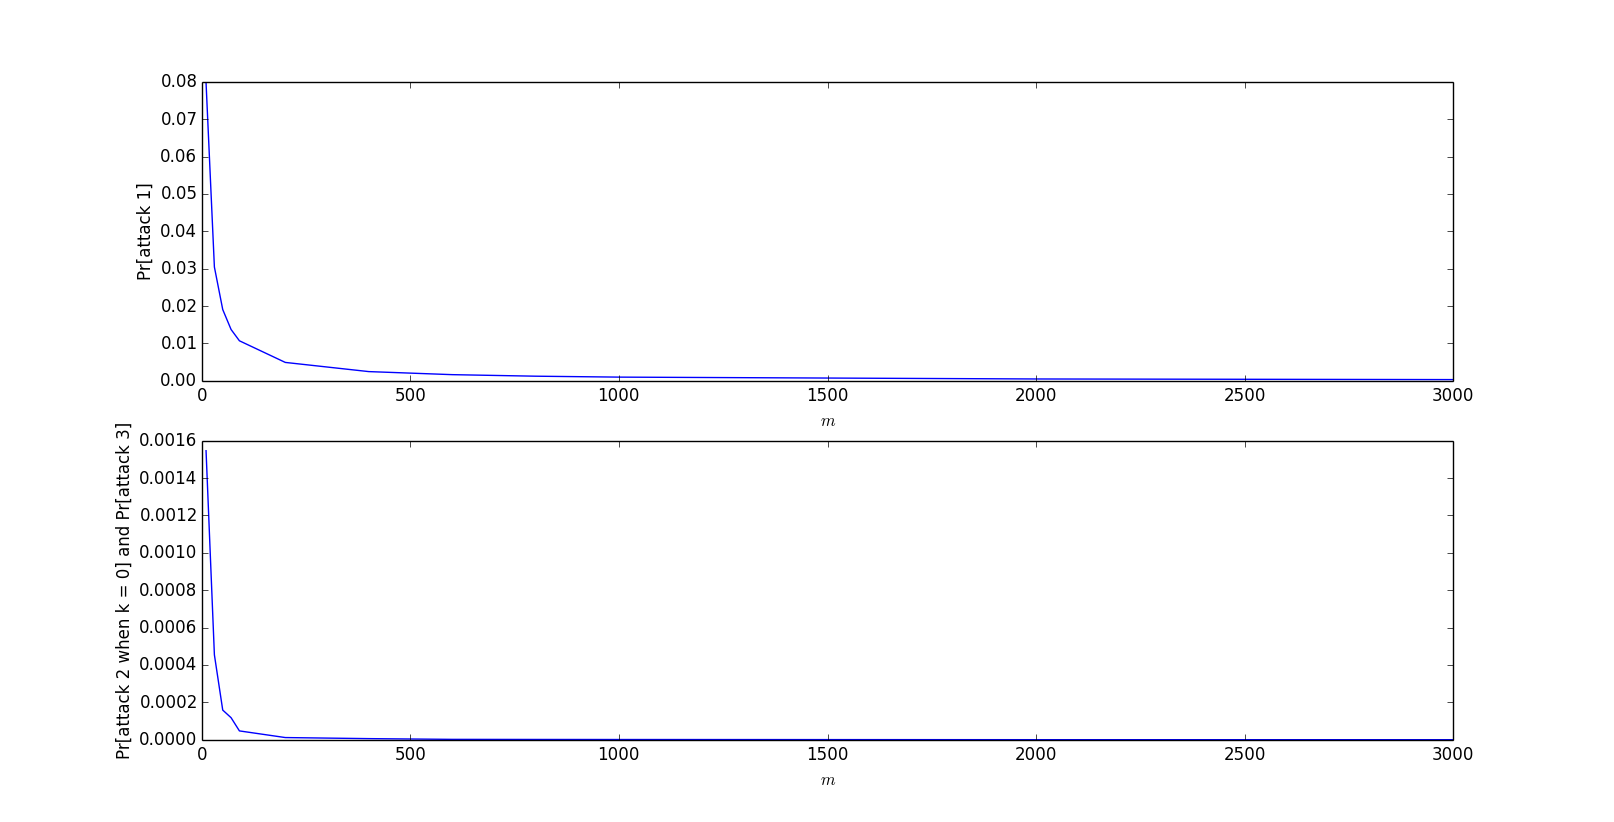
\includegraphics[width=16cm]{images/attack123.png}
	  \caption{The success probabilities of attack 1, 2 and 3}
	  \label{fig:attack123}
\end{figure}


We give the total attack probabilities (i.e., $p'_X\pr[\mathsf{attack X}]$)is given in the Figure \ref{fig:total}. As it can be seen the success of the attacks are very low. Remember that all these attacks can be happen when all parachain validators are malicious. So, in this case, they have this probability. Otherwise their success probabilities are 0.

\begin{figure}[h]\centering
	  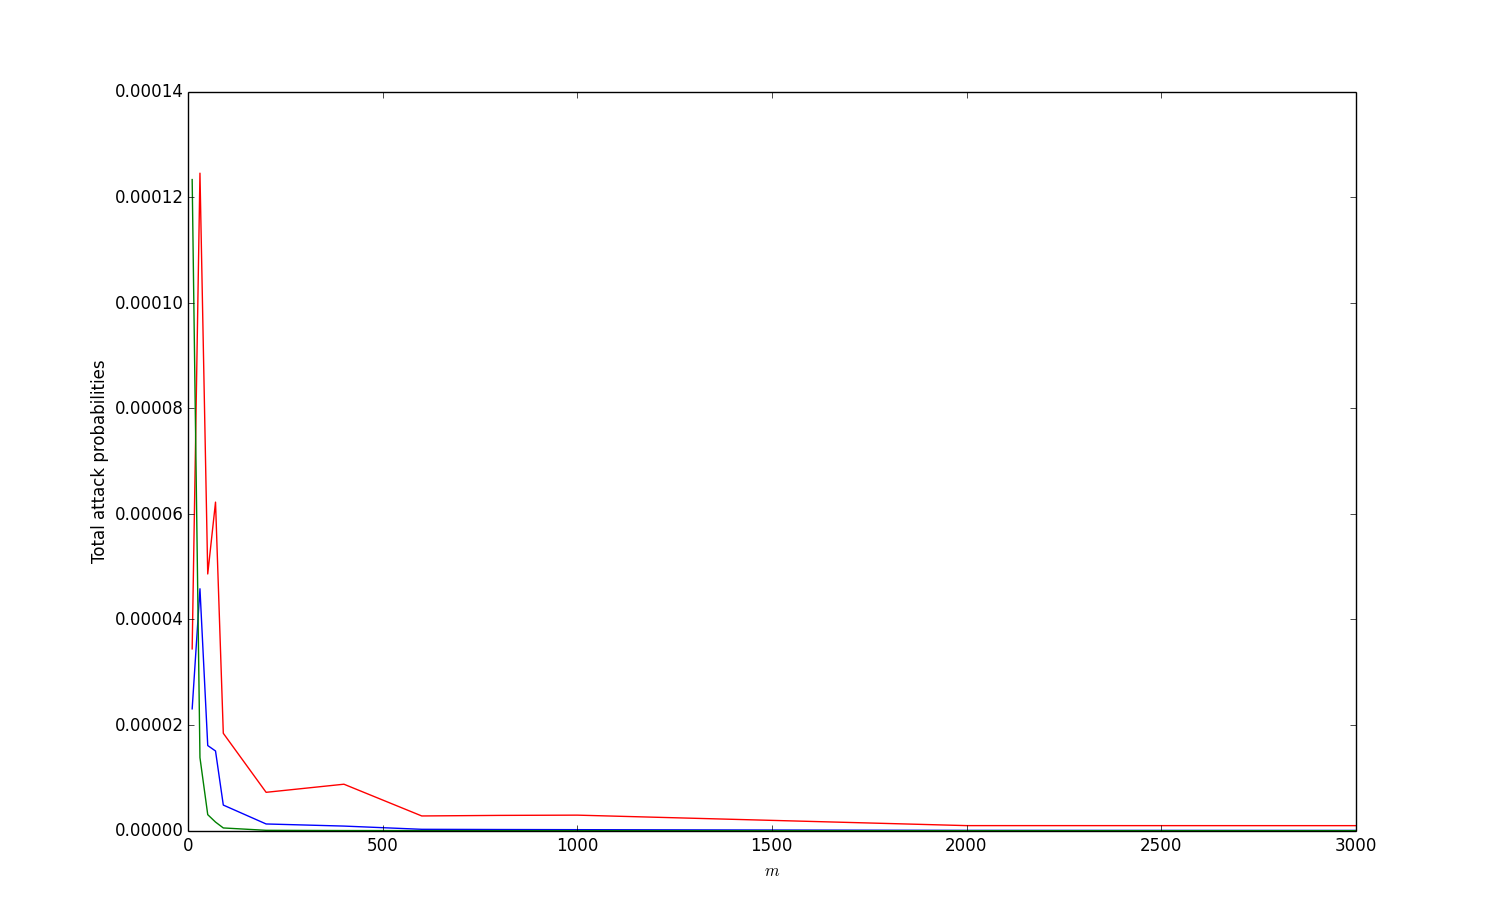
\includegraphics[width=16cm]{images/totalattack.png}
	  \caption{The total attack probabilities. Red is for attack 1, blue is for attack 2 and green is for attack 3.}
	  \label{fig:total}
\end{figure}




% We first compare the conditions to execute the attack 1, attack 2 and attack 3. The condition for attack1 is to have at least $\mu$ malicious validators satisfying the the condition (\ref{cond:mod}) which is given in the probability below:






% The attack 3 condition is to have no honest validator satisfying the condition (\ref{cond:mod}) and it probability is:

% \begin{equation}\label{eq:att3cond}
%     p'_3 = \pr[\text{no honest in condition (\ref{cond:mod})}] = (1-\frac{1}{m})^{2n/3}
% \end{equation}


% When we compare $p'_1, p'_2$ and $p'_3$ (See equations (\ref{eq:att1cond}), (\ref{eq:att2cond}) and (\ref{eq:att3cond}), respectively), we see that $p'_2$ is the greater than the others. Therefore, we choose the parameter $\mu$ according to $p'_2$ to make $p'_2$ is very small so $p'_1$ and $p'_3$ too. 

% First, let's analyze the probability of attack 1 which depends only $n/m$ to find a relation between $n$ and $m$ with using equation \ref{eq:attackgain}. Then, we obtain

% \begin{equation}\label{eq:relation}
%     n > \frac{3m\ln(m+1)}{2}
% \end{equation}

% If we preserve this relation then the attack 1 (and so attack 2 and attack 3) will be small enough so that the adversarial gain from this attack is small comparing to his lost.

% Now, consider the case where all parachain validators are malicious and assume that the set of parachain validators changes in each epoch. In this case, the probability of satisfying the necessary condition in one slot to execute attack 1 should be less than $\frac{1}{\zeta}$ where $\zeta$ is the expected number of malicious slots in one epoch. According to  \href{http://research.web3.foundation/en/latest/polkadot/BABE/Babe/#6-practical-results}{BABE practical results} (e.g., $c = 0.034, T = 3$ and $k = 54$ ), the epoch length should be around 20000 slots and expected number of malicious slots are around 215.  


% \begin{figure}[h]\label{fig:muval}\centering
% 	  \includegraphics[width=8cm]{muval.png}
% 	  \caption{The parameter $\mu$ according to number of parachains}
% \end{figure}


% Analysis of attack 2 is different than attack 1 because for this attack, the adversary do not need to wait for satisfying a specific condition (e.g., for attack 1, the adversary should wait for the block where at least $\mu$ malicious validators satisfy the condition (\ref{cond:mod})). The reason of this is that there exists always a $k \in \mathbb{N}$ which let at least $\mu$ malicious validators being selected for the extra check in every block. When the adversary executes the attack 2, we assume that $x < \mu$ malicious validators satisfy the condition (\ref{cond:mod}) and at least $\mu - x$ malicious validator satisfy the condition (\ref{cond:time}) until the time $\tau_k$. The best case for the adversary in order to have the lowest probability in attack 2 (See (\ref{eq:attack2})) is when $k = 0$. Therefore, the best case probability needs to be less than $1/\zeta$ for all $x$. The best case probability is the following:

% \begin{equation}\label{eq:bestcaseinatt2}
%     \pr[\text{best  case for }\mathsf{attack 2}] = \sum_x^{\mu-1}\binom{f'}{x}\frac{1}{m^{x}}(1-\frac{1}{m})^{f'-x}\sum_{i = \mu-x}^{f'}(\frac{\mu}{n-n/m})^{i}(1-\frac{\mu}{n-n/m})^{f'-i}
% \end{equation}

% If we choose  the parameter $\mu$ as in Figure \ref{fig:muval}, the best case probability will be greater than $1/\zeta$ as it can be seen in Figure \ref{fig:bestforattack2}. It means that when parachain validators are malicious, they have more chance to execute the attack 2 during their period. However, the probability of executing the attack 2 is much smaller than attack 1 probability which less than $1/m$. It means that it is too risky for the adversary to execute attack 2 considering the risk function in Equation (\ref{eq:attackgain}).

% \begin{figure}[h]\label{fig:bestforattack2}\centering
% 	  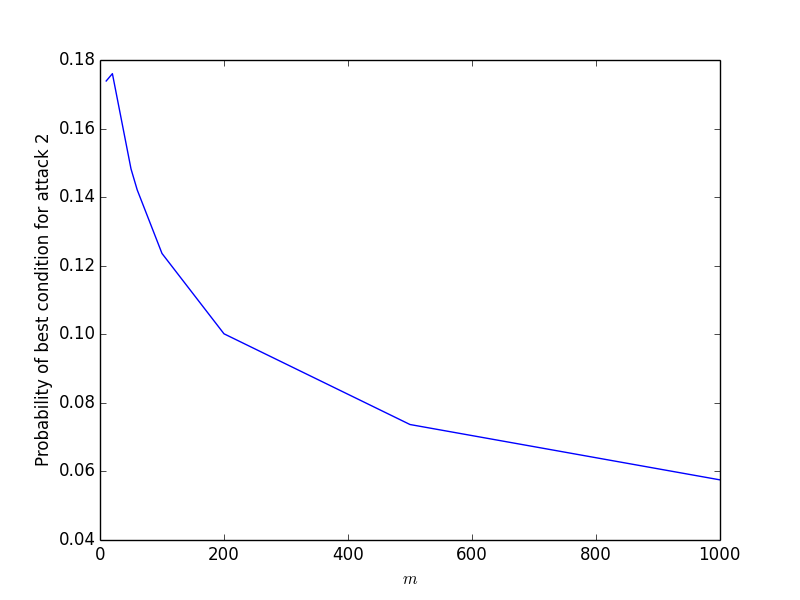
\includegraphics[width=8cm]{bestcond.png}
% 	  \caption{The probability of having the best case for attack 2.}
% \end{figure} 

% Lastly, we analyze attack 3. The attack 3 condition is to have no honest validator satisfying the condition (\ref{cond:mod}). In the analysis of attack1, we fix it to $1/m$. Similar to attack 2, if $m < \zeta$, hen parachain validators are malicious, they have more chance to execute the attack 3 during their period. With the same probability as in attack 2, executing attack 3 is too risky for the adversary considering its gain and lost.

% The total attack probabilities is given in the graph below:

%If the number of parachain increases, we can see that the probability of having all parachain validators malicious decreases. However, the probability of  condition for attack 1 (See equation \ref{eq:attack1cond}) increases when $m$ increases if $\mu$ is constant. Therefore, the parameter $\mu$ needs to be selected according to number of parachains.






% The adversaries satisfies the condition to execute the attack if at least $\mu$ malicious validators are in condition (\ref{cond:mod}). Given a fixed number of parachain, if number of validator increases then the probability in \ref{eq:cond1} increases. On the other hand, the probability of attack1 decreases. Therefore, in this case, we need to find $n/m$ which makes attack 1 probability low enough and according to this find a $\mu$ value which make \ref{eq:cond1} low enough.


% The condition for attack 1 is to have $\mu'$ malicious validators in the condition (\ref{cond:mod}). This condition happens with probability $\binom{f'}{\mu'}\frac{1}{m^{\mu'}} $.
% We do not have any condition for attack 2.
% The condition of attack 3 is that there is no honest party satisfying condition $(\ref{cond:mod})$. This happens with probability $\pr[\mathsf{attack1}] \leq \exp(-\frac{2n}{3m})$.


% So, first of all we need a relation between $n$ and $m$  so that the probability of attack 1 is small enough so that attack 2 and attack 3. Considering the economics of the entire protocol, this probability needs to be smaller than $1/m$. In this case, we have the following relation between $n$ and $m$:

% \begin{equation}\label{eq:nm}
%     n > \frac{-3m\ln(m^{-1})}{2}
% \end{equation}


% In addition, the good conditions for attack 1 needs to be small enough so that the adversaries won't have many chances to execute attack 1.




% There are certain parameters that we need to fix to make sure the security of the protocol. 


% Remark that attack 1 (See inequality (\ref{eq:nocond1})) only depend of number of parachain  validators $n/m$.  As it can be seen in Figure \ref{fig:attack1prob}, if the ratio of number of validators and parachain validators are more than 10, the the attack1 probability is very close to 0. Therefore, it is critical to satisfy this ratio to have security.

% \begin{figure}[h]\label{fig:attack1prob}\centering
% 	  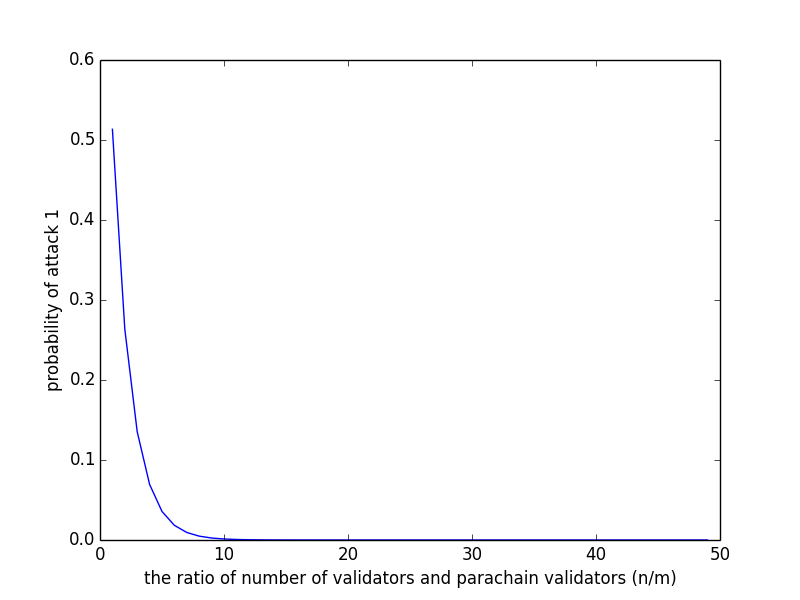
\includegraphics[width=7.5cm]{attack1.png}
% 	  \caption{The probability of attack 1 which depends on $|PV| = n/m$}
% \end{figure}




% In our next analysis for attack 3, we assume that $|PV| = n/m \geq 10$ so $c\geq 10/n$. In our attack 3 analysis, we find the minimum number of extra check $\mu$ for security.
% In the case of all collators are malicious and collaborating with the parachain validators, they prefer to make the blob unavailable to fishermen. Therefore, we cannot rely on fishermen in this case because they will not access the block to check the validity. Besides, we do not receive any unavailability report from collators. Therefore, if all collators are malicious, it makes sense to assume that $\runav + \rinv = 0$, and so $\mu' = \mu$. Even in this case, the above attack probabilities has to be low enough for the malicious parties so that they do not to risk their stake and reputation. In below Figure \ref{fig:attack3prob}, it can be seen that $\mu$ needs to be at least between 8 and 10 in order to have very low attack 3 probability.


% \begin{figure}[h]\label{fig:attack3prob}\centering
% 	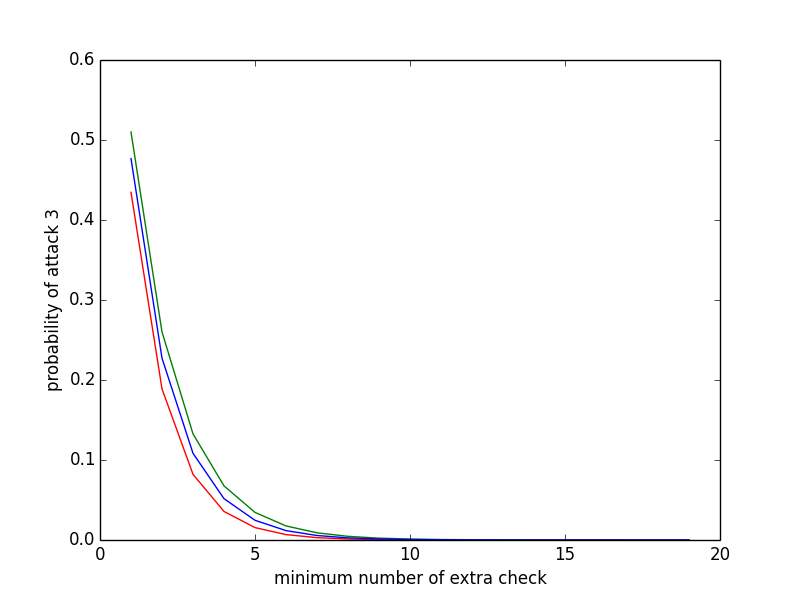
\includegraphics[width=7.5cm]{attack3.png}
% 	\caption{The probability of attack 3 which depends on number of validators and $\mu$. In red graph $n = 50$, in blue graph $n = 100$ and in green graph $n = 1000$.}
% \end{figure}



% In the case where all collators are not malicious, we can rely on the unavailability reports from collators.
\section{Security of Availability and Validity}


\begin{theorem}[Availability]
Assuming the Merkle tree constructed from collision resistant hash functions and a block in GRANDPA can be finalized with at least $2f+1$ votes, then the availability protocol is secure.
\end{theorem}

\begin{proof}
Assume that an unavailable block is finalized. It means that this finalized block includes a block header of which at most $f$ honest validators has the correct erasure code piece (See Definition \ref{def:unavail}). If this block is finalized, it means that
\begin{itemize}
    \item either not all honest validator who does not have the erasure code piece announce the unavailability. If they would announce it, since their number is at least $2f+1 - f =f+1$ (i.e., honest parties - honest parties who do not have the erasure code), the other honest parties do not finalize it and malicious parties do not have enough number to finalize it. Therefore, we can assume that there is at least one honest party who do not announce the unavailability of its erasure code in this case, because he thinks that he has one but actually it is not correct. If there exists a one honest party who has incorrect erasure code, but having the proof that it is correct (provided by parachain validators), then it means that the collision resistance assumption of Merkle tree is broken. 
    
    \item or  $f+1$ parties announces unavailability it means that GRANDPA finalize the block with at most $2f$  parties. So, this implies that the security of GRANDPA is broken by finalizing a block with less than $2f+1$ votes.
\end{itemize}

Since the GRANDPA is secure and the Merkle tree is collision resistant, the unavailability protocol is secure.
\end{proof}

\begin{theorem}[Validity]
\label{thm:valid}
Assuming that the availability protocol is secure, the signature scheme is EF-CMA secure, the hash function $H$ in Conditions (\ref{cond:time}) and  (\ref{cond:equiv}) is a random oracle, the PoV protocol is secure and correct (Definition \ref{def:pob}), the VRF is secure and a block in GRANDPA can be finalized with at least $2f+1$ votes then the invalid block is finalized in the relay chain with probability less than risk probability.
\end{theorem}

\begin{proof}(Sketch)
TODO: Security reduction, Rewrite the security arguments


If there is one honest $PV$ and there is not any $f+1$ unavailability report, then at least $2f$ of the honest parties has the piece. It means that $PV$ can collect all the pieces from the honest parties in order to reconstruct the blob and check its validity. Therefore, if there is at least one honest party in $PV$, it can detect the invalidity and announces it. In the end, we will have more than $f$ invalidity signatures since the other parties also check invalidity after seeing the signature saying that the block is invalid.

Therefore, all parachain validators have to be malicious not to be caught. 
If there is at least one honest validators who is assigned for extra validity check with either of the conditions then the same case happens as having at least one honest parachain validators. Therefore, an invalid block cannot be detected (the attack succeeds) if all parachain validators are malicious and all extra check validators are malicious. 

Remark that the extra check conditions (\ref{cond:mod}) and (\ref{cond:time})  with $\tau = 0$ and (\ref{cond:equiv}) and (\ref{cond:modequiv}) guarantees that the expected number of checks by parachain validators and the extra check validators is $\vcheck$. %In addition to this, the selection mechanism of parachain and extra check validators  guarantees with a overwhelming probability that each validator is responsible from only one parachain as an either extra-check validator or parachain validator. 
Therefore, we can consider that the parachain validator and extra-validator selection mechanism actually randomly samples $\vcheck$ validators for each parachain. So, the probability of all selected validators for a particular parachain is malicious is bounded by $(\frac{1}{3})^{\vcheck}$. See \ref{lem:permutation} for the details.

\end{proof}



\begin{theorem}\label{thm:vcheckmal}
Given that $\vcheck$ malicious validators are eligible to check the validity of a block header, the invalidity attack is bounded by the probability  $\exp(-\frac{2}{3}(\mu+r))$ if $\mu + r < n/m$ and the probability $\exp(-\frac{2n}{3m})$ if $\mu + r \geq n/m$.
\end{theorem}

\begin{proof}

Below, we give the probability of any validator being in conditions (\ref{cond:mod}), (\ref{cond:time}), (\ref{cond:modequiv}), (\ref{cond:equiv}):

$$\pr[\text{Cond. (\ref{cond:mod})}] =\pr[\text{Cond. (\ref{cond:modequiv})}] = p_{vrf} = \frac{1}{m}$$
$$\pr[\text{Cond. (\ref{cond:time}) at time } \tau] = p_\tau =  \frac{\mu'}{n - nc} + \tau $$
$$\pr[\text{Cond. (\ref{cond:equiv}) }] = \frac{\mu'}{n - nc} $$


We assume that $|\pv| = \frac{n}{m}$.  The number of $\vcheck-|\pv| = \mu + r$ malicious validators can be selected for the extra check  with the following cases:

\begin{enumerate}
    
    \item $\mu + r \geq \frac{n}{m}$ and at least $\mu + r$ malicious validators are in condition (\ref{cond:mod}) and condition (\ref{cond:time}) until the time $\tau_k$ for the parachain whose validator are malicious. The attack probability is highest if at least $\mu + r$
    malicious validators are in (\ref{cond:mod}). In this case, the attack succeeds if no honest validator satisfies the condition (\ref{cond:mod}) 
    
    
    \begin{align}\label{eq:attack2}
        \pr[\mathsf{attack1}] &= (1-\frac{1}{m})^{2n/3} <  e^{-2n/3m} \nonumber
    \end{align}
    
    
    \item $\mu+r < \frac{n}{m}$ and at least $\mu' = \mu+r$ malicious validators are in condition (\ref{cond:time}) until the time $\tau_k$. For simplicity, we divide time in discrete values $[\tau_0 = 0, \tau_1 =u, \tau_2 = 2u, ..., \tau_k = ku]$. $\tau_k$ can be computed by malicious validators before the validation process begins. The probability of this attack is the following
    
    \begin{align}
        \pr[\mathsf{attack2}] &= \prod_{i = 0}^k(1-p_{\tau_i})^{\frac{2n}{3}} \nonumber\\
        &\leq  \prod_{i = 0}^k (1 - \frac{\mu'+\tau_in(1-c)}{n(1-c)})^{\frac{2n}{3}} \nonumber\\
        &=  \exp(\sum_{i = 0}^k -\frac{2}{3}\frac{\mu' + \tau_in(1-c)}{1-c}) \nonumber\\
        & = \exp(-2/3(\frac{(k+1)\mu'}{1-m/n}+ nu\frac{k(k+1)}{2})\nonumber
    \end{align}
    Remark that $\pr[\mathsf{attack3}]$ is maximum when $k = 0$. When $k = 0$, $\pr[\mathsf{attack3}] \leq \exp(-\frac{2\mu' n}{3(n-m)}) \leq \exp(-\frac{2}{3}(\mu + r))$.
    x
    
    \item This case considers equivocation: Here, we can assume that the adversary knows who satisfies the condition (\ref{cond:mod}) and (\ref{cond:time}) since if the malicious validator is the block producer, he first produces the block and sees who validates this block. If no honest validator checks it with condition (\ref{cond:mod}), he equivocates it. When this happens, the attack succeeds if no honest party satisfies the condition (\ref{cond:modequiv}) or (\ref{cond:equiv}). Hence,
    the probability of attack 4 is
    
    \begin{align}
    \pr[\mathsf{attack} 4] &=\pr[\text{no honest check in  cond. (\ref{cond:equiv}) and (\ref{cond:modequiv})}]\nonumber \\ 
							&\leq \pr[\mathsf{attack1}](1-\frac{\mu'}{n-nc)}) ^{\frac{2}{3}n} \nonumber\\
				            & \leq \exp({-2/3(\frac{n}{m}+\mu + r)}) \nonumber
    \end{align}
\end{enumerate}	
    % \item  In this attack, the adversary equivocates and it does it when $\mu'> n/m$ and there are $n/m$ malicious adversaries satisfying the condition (\ref{cond:mod}). we can assume that the adversary knows who satisfies the condition (\ref{cond:mod}) since if the malicious validator is the block producer, he first produces the block and sees who validates this block. If no honest validator checks it, he equivocates it with a block where at least $n/m$ malicious validators satisfies the condition (\ref{cond:modequiv}). Then, the attack succeeds if no honest party satisfies the condition (\ref{cond:equiv}). 
    % The probability of attack 3 is
    
    % \begin{align}
    % \pr[\mathsf{attack}3] &=\pr[\text{no honest check in  cond. (\ref{cond:equiv})}]\nonumber \\ 
				% 					   &\leq (1-\frac{\mu'}{n-nc)}) ^{\frac{2}{3}n} \nonumber\\
				% 					   &\leq e^{-2/3(\frac{\mu'}{1-c})} \nonumber
    % \end{align}
    
    





%
%Therefore, the attack probability is $\pr[\mathsf{attack1}]+\pr[\mathsf{attack2}]+\pr[\mathsf{attack}3]$.



%Here, we consider $r_a = 0$ to compute the maximum attack probability and $c_f' = \lceil r_f \rceil$. We do not take $r_f = 0$, because we assume that there is always at least one fisherman.


%a parachain validator does not know who are the extra-check validators except the malicious validators if they are assigned to extra check. This comes from the VRF security. So , since $H$ is a random oracle, $B$ is derived from a uniform distribution between $[0,1]$. Therefore, the probability of a validator is assigned to be an investigator at time $\tau$ given that not enough validity check (i.e., $|\mathcal{I}| < \vcheck$) is done before $\tau$ is:

%$$p_{\tau} = \frac{\vcheck - |\pv|}{|\V|-|\pv|}+\tau  = \frac{1+\lceil \runav + \rinv \rceil}{n-nc}+ \tau$$

%assuming that $|PV| = nc$ where $c \in (0,1)$.

%Remark that when $\tau$ increases meaning that when the time increases without having sufficient validity check, $p_{\tau}$ increases and reaches 1 at some time. For simplicity, we divide time in discrete values $[\tau_0 = 0, \tau_1 =\mu', \tau_2 = 2\mu', ..., \tau_k = k\mu']$ where $k\mu'$ is the time when the number of malicious parties in $\mathcal{I}$ is $\vcheck$. This time can be computed by malicious validators before the validation process begins. In any case, the only way not to be caught is not to have any honest extra-check validator until $k\mu'$. The probability of this is the following given that  the number of malicious parties in $\mathcal{I}$ is $\vcheck$:

%\begin{align}
% \pr[\mathsf{attack} = 1] = \prod_{i = 0}^k(1-p_{\tau_i})^{2f+1} \leq (1-p_{\tau_0})^{2f+1} &\leq (1-\frac{1+c'_f}{n(1-c)}) ^{\frac{2}{3}n} \nonumber \\
%& \leq e^{-2/3\frac{1+c_f}{1-c}} \nonumber
%\end{align}
%Here, we consider $r_a = 0$ to compute the maximum attack probability and $c_f' = \lceil r_f \rceil$. We do not take $r_f = 0$, because we assume that there is always at least one fisherman.



\end{proof}


\section{Practical Results}

As it can be seen from the proof of theorem \ref{thm:valid}, malicious validators can attack the validity protocol with probability $(\frac{1}{3})^{\vcheck}$. Remember that $\vcheck = |\pv| + \mu + r$ where $r = \lceil r_a + r_f \rceil$. If we assume that parachain validators change in every $x$ minutes, the malicious parties needs to wait $x3^{\vcheck}$ minutes in order to succeed the attack. For example, if $x = 5$ minutes, then the total time for an attack for each $\vcheck$ is given in Figure \ref{fig:totaltime}:


\begin{figure}[h]\centering
	  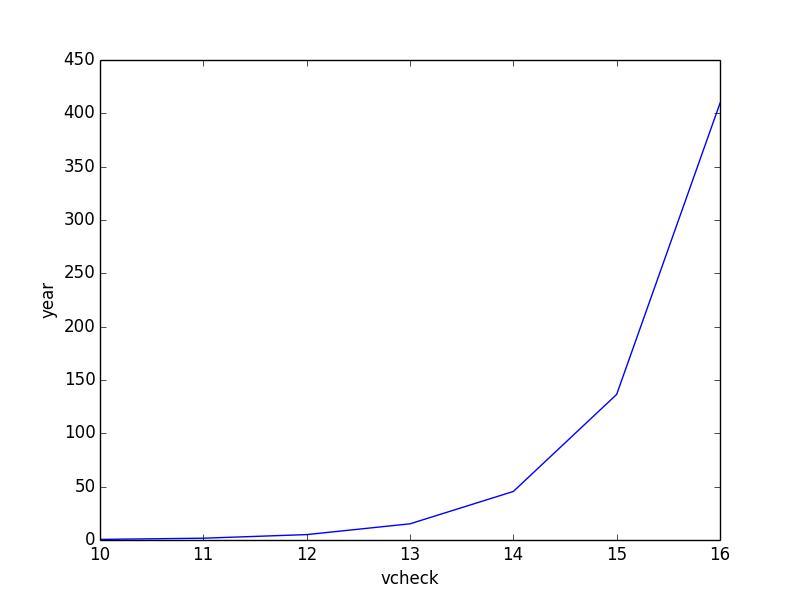
\includegraphics[width=10cm]{images/year.png}
	  \caption{It shows the waiting time for an adversary for a successful attack given that every parachain validators changes every 5 minutes}
	  \label{fig:totaltime}
\end{figure}

As it can be seen that if $\vcheck$ is more than 14, the adversary needs to wait more than 50 years for the attack. Therefore, in terms of security, it is important to have always minimum $\vcheck$ validators.

\paragraph{The parameter $\mu$:} The possible $\mu$ (minimum number of extra check) values:

\begin{itemize}
    \item If $\mu = 0$, then $|pv| = 14$ in order to make sure that minimum $\vcheck$ is always equal to $14$. Given that $|pv| = n/m$ where $m$ is the number of parachain validators $n = 14 * m$. 
    
    \item If $\mu > 0$, then $|pv| < 14$. It means that we need less validators for the security than the case where $\mu = 0$. Less validator implies less network delay and less network delay implies more secure BABE. On the other hand, if $\mu$ increases, it means that more validators need to reconstruct a blob in order to check the validity. So, validators need to do more work. In terms of scalability of the relay chain, we need to decide $\mu$. 
\end{itemize}
In rule of thumb, if we don't care the number of validators as far as it is not the maximum  number of validator ($N$) that Polkadot can handle, then $\mu$ should be if $14 * m < N$ then $\mu = 0$. Otherwise, $\mu = 14 -N/m$. 

Another disadvantage of having $\mu = 0$ is to have less risky attack  when all parachain validators are malicious. Imagine a parachain with a few collators. We can assume that they may be malicious and collaborate with the malicious validators. In this case, the validators will not have any report. So, there will be 0 extra check. As soon as, all parachain validators are malicious for this malicious parachain, they can add invalid block headers and cannot be caught. The security argument says here that they need to wait around 50 years for this, so the attack is not possible. However, in the real life, since the attack does not have any risk, the collators can bribe parachain validators with their stake and parachain validators validate an invalid blob.


Theorem \ref{thm:vcheckmal} gives the risk that  malicious validators put at  when they put an invalid report.  If $\mu + r \leq n/m$, the invalid block will not be detected with probability $\exp(-\frac{2}{3}(\mu+r))$. In the worst case scenario, if no report is received than the attack probability is $\exp(-\frac{2}{3}(\mu))$. We give in Figure \ref{fig:mu} that the probability of successful attack if in the case of $\vcheck$ malicious validators are selected. As it can be seen Figure \ref{fig:mu}, their risk is exponentially increasing when $\mu$ increases. In order to make the risk close to 0 even if no report received, $\mu$ should be greater than $4$.

\begin{figure}[h]\centering
	  \includegraphics[width=12cm]{images/muval.png}
	  \caption{The risk of malicious validators when they attack even if $\vcheck$ validators are malicious}
	  \label{fig:mu}
\end{figure}

\paragraph{Fisherman and Collator Reports:} In the validity scheme, we rely on the invalidity reports of fishermen and  unavailability reports of collators. We also want to total number of $\vcheck$ so that these reports do not make too many validator to check the validity. Total number of extra check can be at most $\mu_{max}$ (i.e, $\mu + \lceil r_f + r_a \rceil \leq \mu_{max}$). This bound is necessary because regular malicious reports can slow down the process easily. 

When a fisherman sends a report of invalidity but later on it is understood that actually it is valid, the fisherman is slashed. Therefore, the reliability of a fisherman report can be measured by how much it is staked. 
Considering this, $r_f$ can be computed as follows:

$$r_f = \frac{\sum_{i}\mathsf{stake}_{f_i}}{v_{gain}}$$

Here, $\mathsf{stake}_{f_i}$ is the stake that a fisherman $f_i$ has for this report and $v_{gain}$ is the dot value that a validator receive in each block. In a nutshell, a fisherman needs to stake at least the same amount that the validator earns for each block in order to make a validator to execute an extra validity check. If the fisherman report is not valid, then the fisherman pays for this extra check. So, malicious fishermen has to spend $\mu_{max} v_{gain}$ every time to make busy with invalidity extra check with the maximum capacity. We believe that this model discourages fishermen to send false reports. 

However, we cannot measure the reliability of unavailability reports as fisherman's reports since it is not possible to show the correctness or incorrectness of any unavailability reports. Malicious collator do not lose anything by just sending fake unavailability reports. In order to solve this issue, we assign a parameter $\alpha \in (0,1)$ for a parachain that defines the proportion of honest collator assumption. Depending on $\alpha$, we have define $r_a$ for two case:
\begin{itemize}
    \item if $\alpha > 1/2$, $r_a = \mu_{max}^{x/\alpha}$ 
    
        \[   
    r_a(x)= 
     \begin{cases}
       \mu_{max}^{x/\alpha} & \text{if } x \leq \alpha \\
       \mu_{max} &\text{otherwise} \\ 
     \end{cases}
\]  
    
    where 
    $$x = \frac{\text{total unavailability reports}}{\text{all collators}} = \frac{\sum_{c_i \in C_P}st_{c_i}}{|C_P|}.$$
    
    Here, $st_{c_i}\in \{0,1\}$ which is 0 if the block is available. Otherwise, it is 1. The reason of using a function such as $\mu_{max}^{x/\alpha}$ is to make sure that we have extra checks close to maximum check only if the number of unavailability reports are close to the number of honest collator assumption. Thanks to this, if number of honest collators are majority, the malicious collators who want to slow down Polkadot cannot achieve to make always maximum number of checks with only unavailability reports. In general, these type of parachains can be investigated by fisherman as far as the blocks are available to honest collators. Therefore, we expect that if there is any invalid block, the fishermen catch it and send a report. If the blocks are unavailable to honest collators (so fisherman), validators checks the invalidity with the maximum capacity.  
    
    \item if $\alpha < 1/2$, then it is important to give more importance to the unavailability reports from this parachain. Therefore, we use the following linear function:
    
    \[   
    r_a(x)= 
     \begin{cases}
       \mu_{max}\frac{x}{\alpha} & \text{if } x \leq \alpha \\
       \mu_{max} &\text{otherwise} \\ 
     \end{cases}
\]  
\end{itemize}

So, $\mu' = \mu + \lceil r_a + r_f \rceil$ if $\mu + \lceil r_a + r_f \rceil \leq \mu_{max}$. Otherwise, $\mu' = \mu_{max}$.


\paragraph{The parameter $\mu_{max}$:} Given the fact that we have maximum number of extra check when there are many invalidity or unavailability  reports, the parameter $\mu_{max}$ needs to be big enough so that the probability of having at least one honest extra check is almost 1.
This probability can be bounded by $1-(\frac{1}{3})^{\mu_{max}}$. Therefore, we can have $\mu_{max} = 15$.

In Figure \ref{fig:ra}, we compute the number of extra checks required depending on the $\alpha$-parameter of a parachain. As it can be seen, the parachain that we trust less requires more extra-checks. The parachain where we assume honest majority reaches the maximum check when the unavailability reports are close to number of honest collators.  


\begin{figure}[h]\centering
	  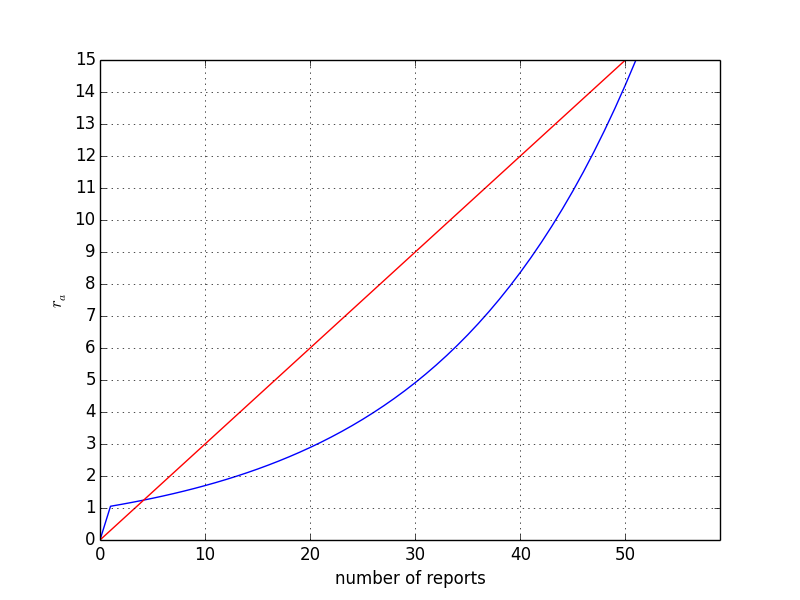
\includegraphics[width=10cm]{images/ra.png}
	  \caption{The red and blue graph shows the number of required extra checks when $\alpha \leq 1/2$ and $\alpha > 1/2$. Here, we assume that the total number of collators are 100.}
	  \label{fig:ra}
\end{figure}



\appendix
\section{Proof Details}

\begin{lemma}\label{lem:permutation}
For any slot number $s$, block producer $bp$, epoch randomness $r$ for the epoch that includes $s$, integer $k >0$, and parachain $P$, with probability at least $1-(f/n)^{-k}$ over the epoch randomness and the random oracles for the hashes and VRFs, for any block that $bp$ produces in slot $s$ that includes a parachain header from $P$, if we eventually have $\vcheck \geq k$ for this parachain header, then some honest validator checks the parachain block.
\end{lemma}
\begin{proof}
Consider generating an ordering $\ell$ of validators as follows, first we have the parachain validators in a uniformly random order, then all validators who satisfy condition (\ref{cond:mod}) (using $bp$'s VRF for slot $s$) in a uniformly random order, then we order all remaining validators in increasing order of the hash $H(ID_{PC} || \mathtt{VRF}_{\sk^v_j}(V))$ used in condition (\ref{cond:time}), breaking ties due to collisions in a uniformly random order. We claim that distribution of $\ell$ is as a uniformly random permutation of the validator set. To see this note that the only operation for which the different validators are treated differently are the VRFs and we assume that they are random oracles. The parachain validators are a set of $n/m$ validators chosen uniformly at random using $r$. Each validator satisfies condition (\ref{cond:mod}) with the same probability independently and so the distribution of the set of validators satisfying (1) conditioned on its size is a set of that size chosen uniformly at random from the non-parachain validators. Also the hashes in (2) are independently and identically distributed.

Next we show that for any block $bp$ produces in slot $s$ which includes a parachain header for $P$,  if any honest validator ever sees that $\vcheck \geq k$, then any honest validators in the first $k$  validators in $\ell$ eventually check that block. All honest parachain validators and honest validators who satisfy (\ref{cond:mod}) check. If all honest validators in the fist $k$ validators in $\ell$ satisfy these conditions we are done. So suppose that $v$ is an honest validator in the first $k$ validators in $\ell$ who doesn't satisfy either of these conditions. $v$ will still check if $\tau$ is large enough and they don't see attestation from $\vcheck$ validators who either are parachain validators, satisfied condition (\ref{cond:mod})  or had a smaller hash in condition (\ref{cond:time}). But noting that all such validators are before $v$ in $\ell$ so there can be at most $k-1$ of them. Thus $v$ only ever counts $k-1$ attestations towards the number needed $\vcheck$ which is eventually $\geq k$. So when $\vcheck \geq k$ and $\tau$ is large enough, $v$ checks.

Finally we need to show that the probability that the first $k$ validators in $\ell$ are honest is at least $(f/n)^k$. Since the first $k$ validators in $\ell$ are distributed as a set of $k$ validators chosen uniformly at random, this probability is $\prod_{i=0}^{k-1} (f-i)/(n-i) \leq (f/n)^k$.
\end{proof}

\end{document}
